\documentclass[11pt, oneside]{article}   	
\usepackage[left=26mm,top=26mm,right=26mm,bottom=26mm]{geometry}    
\geometry{a4paper}                   		
\usepackage{graphicx}			
\usepackage{amssymb}
\usepackage{hyperref}
\usepackage{cite}
\usepackage{url}
\usepackage[parfill]{parskip}
\setlength{\headsep}{5pt}
\graphicspath{ {images/} }


\title{\vspace{-1.6cm}Description of the Basic System}
\author{\textit{An app for visualisation of avalanche hazard}}
\date{}							
\begin{document}
\maketitle

\section{Structure of the Visualisation System}

The application developed for this project consists of user-facing programs (represented by ovals), servers providing real-time data (represented by rectangles) and data computation programs (represented by hexagons), as shown in the followed system diagram.

\begin{figure}[h]
\centering
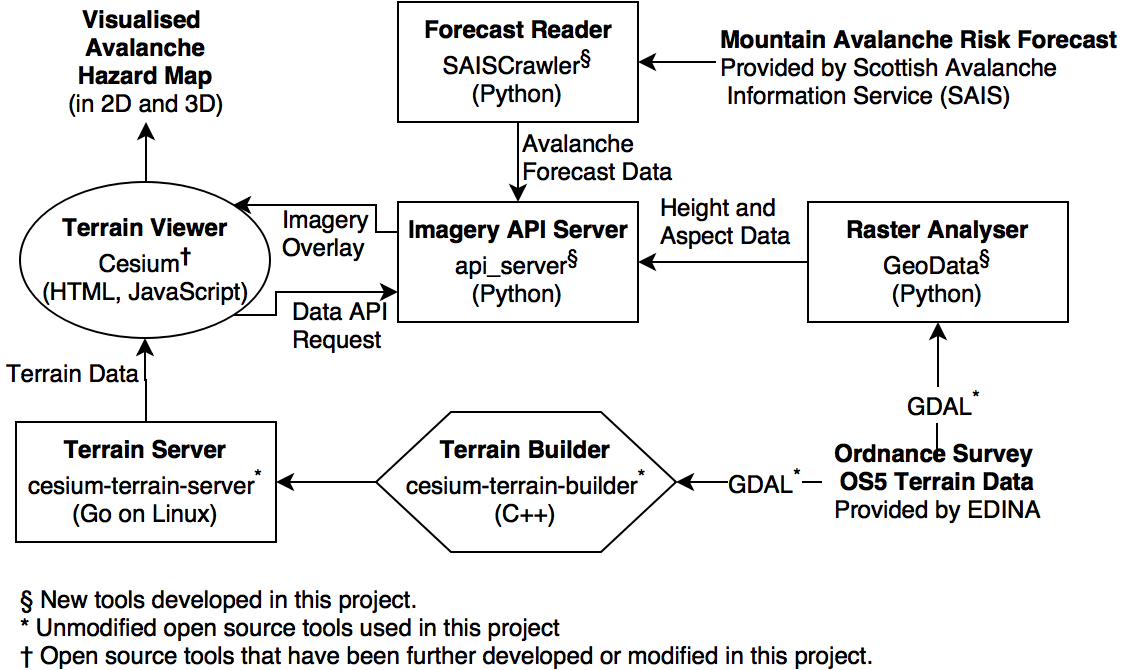
\includegraphics[scale=0.3]{System.png}
\caption{A diagram illustrating the structure of the visualisation system.}
\end{figure}

In order to properly process and visualise data from various sources to the user, several new tools have been developed to complete the tool chain, which also includes a number of existing open source tools, such as GDAL\cite{GDAL} and the Cesium Terrain Builder \cite{cesium-terrain-builder}. The data processing and visualisation processes will be covered in more detail in the next few sections.

\section{Procurement and Processing of Terrain Data}
	For the basic system, height and terrain aspect data is required for geographical areas of visualisation. Although the application is developed based on the availability of avalanche risk forecasts for Scottish Highlands, with the appropriate avalanche risk forecasts and terrain data, this application can be trivially adapted for other mountainous areas.
	
	\subsection{Choice of Data Source}
		There are a number of available sources for Digital Elevation Model (DEM) data of the United Kingdom, most notably the EU-DEM Data \cite{eu-dem} provided by the European Commission and the UK Government's Ordnance Survey Data (OS5) \cite{os-5}, provided free for education by EDINA. 
		
		The EU-DEM Data covers the entire Western Europe with an accuracy of 25 to 30 meters, arranged in the EPSG:3035 \cite{epsg-3035} spatial reference system. The data is available in full, and can be used for both educational and commercial purposes subject to citation requirements. 
		
		The Ordnance Survey (OS5) Data covers the United Kingdom only, with a superior accuracy of 5 meters, arranged in the British National Grid \cite{osgb-1936} reference system. The data can be requested per-tile either for a fee (no usage restrictions) or free through EDINA (educational uses only), subject to citation requirements.
		
		With considerations on the nature of the project and the potential uses of the application, the Ordnance Survey Data is used for the course of the project, as an elevation model with higher accuracy is beneficial for accurate computations and evaluations. However, should an expansion of coverage or usage be required, the EU-DEM Data can be processed and used with the same procedures.
		
	\subsection{Processing of Data} 
		Differing from EU-DEM, the Ordnance Survey Data is supplied on a tile-by-tile basis. Therefore to improve processing efficiency, the first part of the processing procedues is to merge the data into a single GeoTIFF \cite{geotiff} file with the GDAL tool:
		\begin{verbatim}
			find ./OS5/ -name '*.tif' | xargs gdal_merge.py -of GTiff -o OS5_Merged.tif 
		\end{verbatim}
		
		The merged DEM data is then reprojected by GDAL into the WGS84 geodetic system \cite{wgs84} that is used by the majority of mapping and navigation systems:
		\begin{verbatim}
			gdal_translate -a_srs EPSG:4326 -of GTiff OS5_Merged.tif OS5_WGS84.tif
		\end{verbatim}
		
		The reprojected elevation raster \textbf{OS5\_WGS84.tif} can now be used to look up altitude for each point in the geographical area covered by the DEM Data. However, in order to obtain a dataset of terrain aspects for each point within the same boundaries and reference system, it is also necessary to produce an aspect raster, \textbf{OS5\_WGS84\_Aspects.tif} from the elevation raster:
		\begin{verbatim}
			gdaldem aspect OS5_WGS84.tif OS5_WGS84_Aspects.tif -of GTiff
		\end{verbatim}
		
	\subsection{Retrieval of Processed Data}
		Two potential designs have been considered for the implementation of terrain data retrieval: a direct raster lookup system or a database-driven system. 
		
		A brief attempt has been made to build a key-value storage based on MongoDB\footnote{MongoDB: https://www.mongodb.com/}, with geodetic coordinates as key and taking advantage of MongoDB's geospatial system \cite{mongodb-spatial}. However, further evaluations found that although this system provides great flexibility in modifying stored data, in addition to a storage space overhead of approximately five fold, the performance of batch retrieval is insufficient for the data size involved in live operation. Therefore, this implementation has been dropped in favour of the direct raster lookup system.
		
		The direct raster lookup system (\textit{GeoData}) is built to the requirements of high-volume data retrieval, programmed with the Python bindings of the GDAL library. It operates directly on the raster files, and can read ranges of data points efficiently without the need of reading the raster into memory, due to the location-deterministic nature of the GeoTIFF format.  The data retrieval process of this system is illustrated as follows:
		\begin{figure}[h]
		\centering
		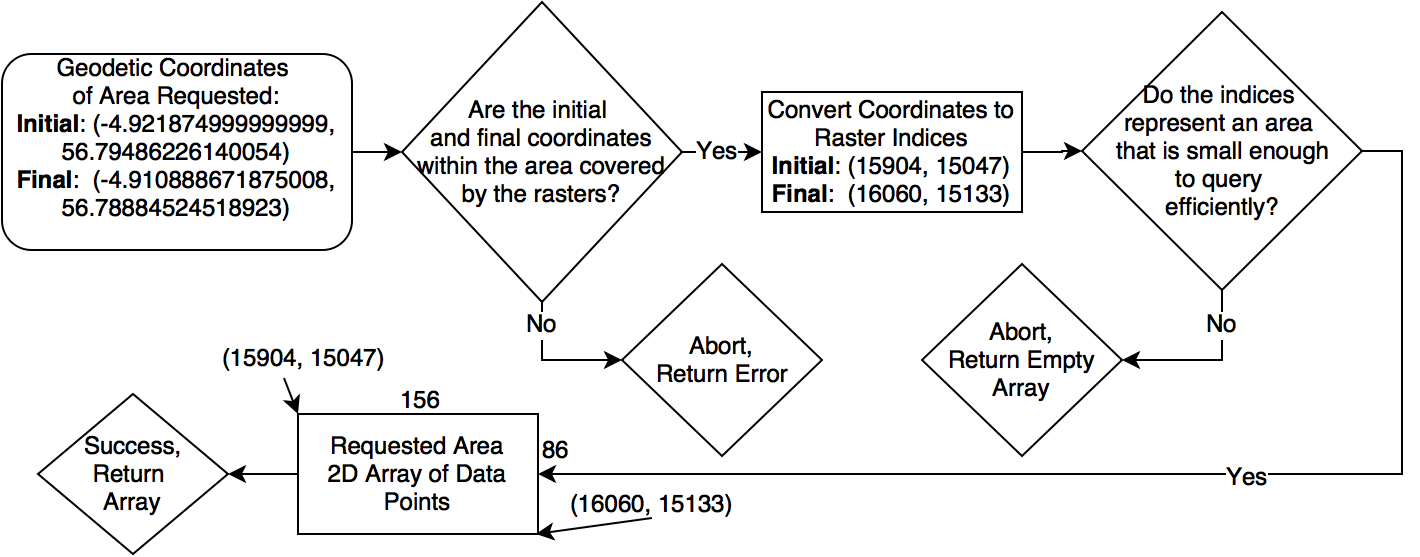
\includegraphics[scale=0.3]{Retrieval.png}
		\caption{A diagram illustrating the retrieval of altitude and aspect data from their respective rasters with geodetic coordinates.}
		\end{figure}
		
		The geodetic coordinates required to retrieve the data would be supplied by the user interface through the \hyperref[sec:APIServer]{Imagery API Server}.
		
		
\section{Procurement and Processing of Avalanche Forecast Data}
	\subsection{Retrival of Forecast Data}
		The Scottish Avalanche Information Service (SAIS)\cite{sais} provides forecasts and information of the avalanche risks in Scottish Mountains several days a week during the winter sport season. The most prominent scale of risk is the hazard compass rose \cite[p. 4]{sais-report}, as shown in Figure \ref{fig:comassrose}. Although not completely representing the risk assessment by itself, it provides an excellent source of information in correlating altitude and aspect to the approximate level of avalanche risk, which can be used as part of a data model in estimating avalanche risk.
		\begin{figure}[h]
		\label{fig:comassrose}
		\centering
		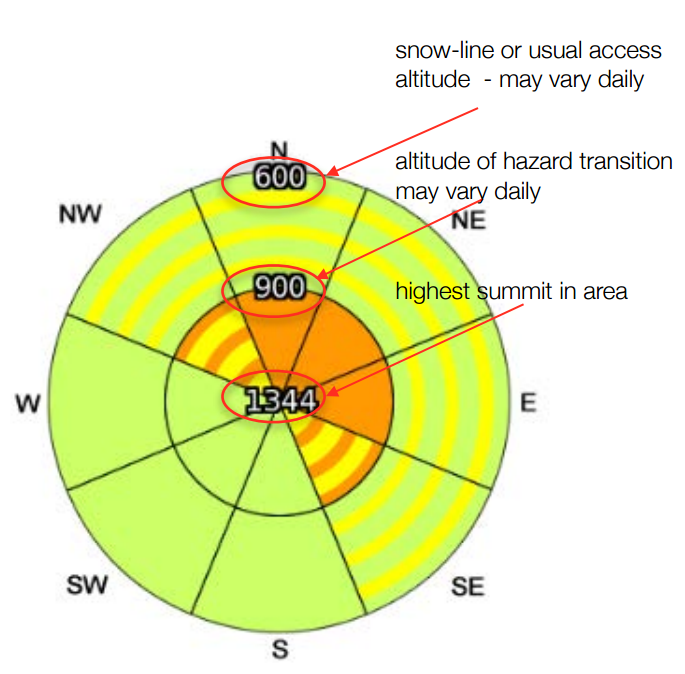
\includegraphics[scale=0.3]{CompassRose.png}
		\caption{An example compass rose produced by the SAIS.\cite[p. 4]{sais-report}}
		\end{figure}
		
		Unfortunately, the SAIS does not provide an API with which the risk levels making up the compass rose could be retrieved easily. Therefore, it was necessary to build a web crawler (\textit{SAISCrawler}) with the Selenium library \footnote{Selenium: http://docs.seleniumhq.org/} to automatically search for and download avalanche forecasts from the SAIS.
		
		The crawler retrieves forecast data by visiting a predefined list of SAIS location pages, each corresponding to a location under observation, and then locate a list of forecasts conducted for that locationn. Each forecast has a unique page containing the image link to the compass rose for the forecast, and the URL encoding of the image link contains the altitude thresholds and risk levels that can be stored. 
		
	\subsection{Structure and Storage of Forecast Data}
	
		Vertically, the forecast data is divided by altitude into two sectors, each of which is further divided by terrain aspect into eight sections, each represents a 30° circular segment, as depicted in Figure \ref{fig:comassrose}. Each segment contains two risk levels: the primary level and the secondary level. In total, there are 16 integer values representing the approximate risk levels of different altitudes and  aspects. These ordered values, along with the forecast date and the three cut-off altitudes are stored in the SQLite database \footnote{SQLite: https://sqlite.org/} by the crawler.
		
		A Python database interface for the SQLite database has been included with \textit{SAISCrawler} for the data to be retrieved by other parts of the application.

\section{Construction and Presentation of the 3D Terrain Model}

\section{API Interfacing of Back-end Systems and User Interface} \label{sec:APIServer}
		
		
		
\bibliographystyle{IEEEtran}
\small{\bibliography{project}}
\end{document}  